\documentclass[a4paper,11pt]{report}
\usepackage{graphicx}
\usepackage{epsfig}
\usepackage{psfrag}
\usepackage{psfrag}
\usepackage{a4wide}
\linespread{1.6}
\begin{document}
\tableofcontents
\appendix
\chapter{MyriaNode}
\begin{figure}[!h]
 \centering
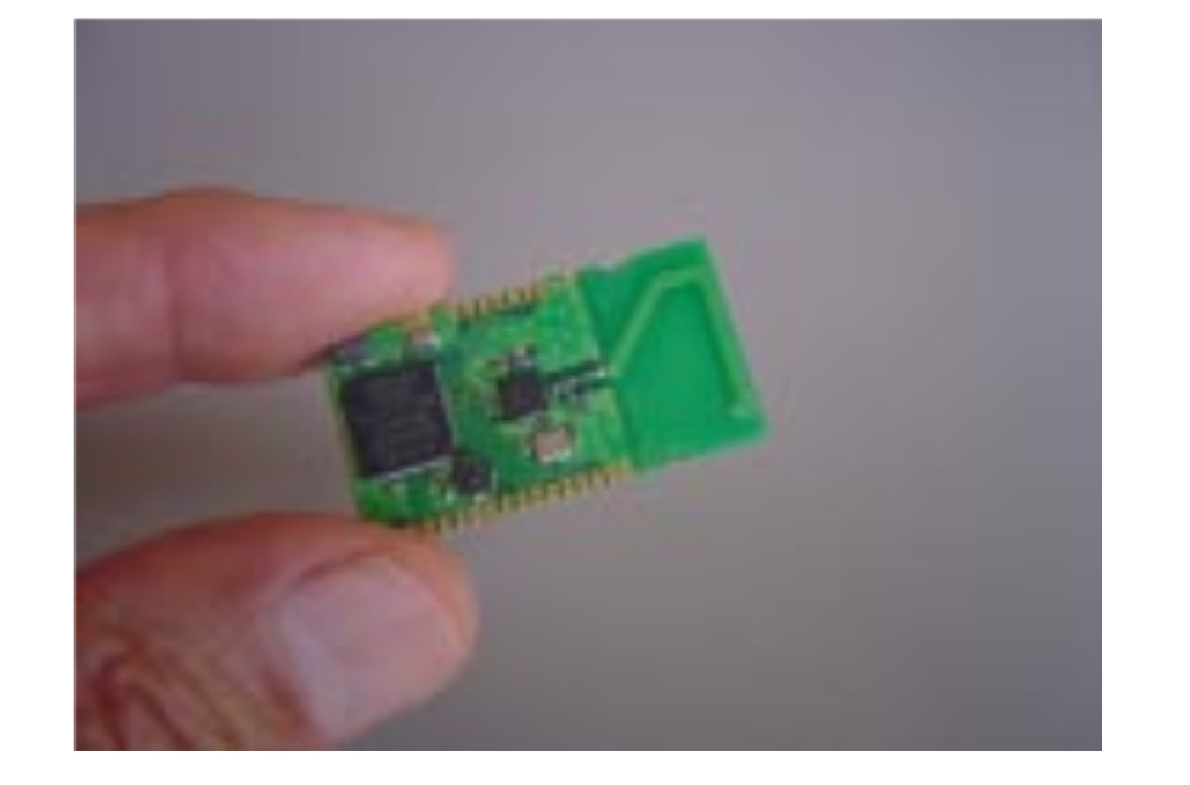
\includegraphics[width=0.5 \textwidth]{myrianode}
\caption{MyriaNode v2.0}
\label{myrianode}
\end{figure}
\subsection{Features}
\begin{itemize}
 \item 2.4 GHz ISM band
 \item Nordic nRF24L01 Radio
 \item Integrated 1/4$\lambda$ PCB antenna
 \item ATMega645 processor
 \item 64kB FLASH
 \item 4kB SRAM
 \item 2kB EEPROM
 \item 32kHz Crystal clock
 \item Size: 20 X 40 mm
 \item Single supply voltage: 1.9V - 3.6V
\end{itemize}
\subsection{Description}
This Wireless Sensor Node is the second generation product for the MyriaNed project. It integrates a Nordic radio module, antenna and embedded processor
all on a PCB. The module is equipped with the software modules as they are being developed by one or more of the working groups of MyriaNed.
\subsection{Architecture}
\begin{figure}[!h]
 \centering
 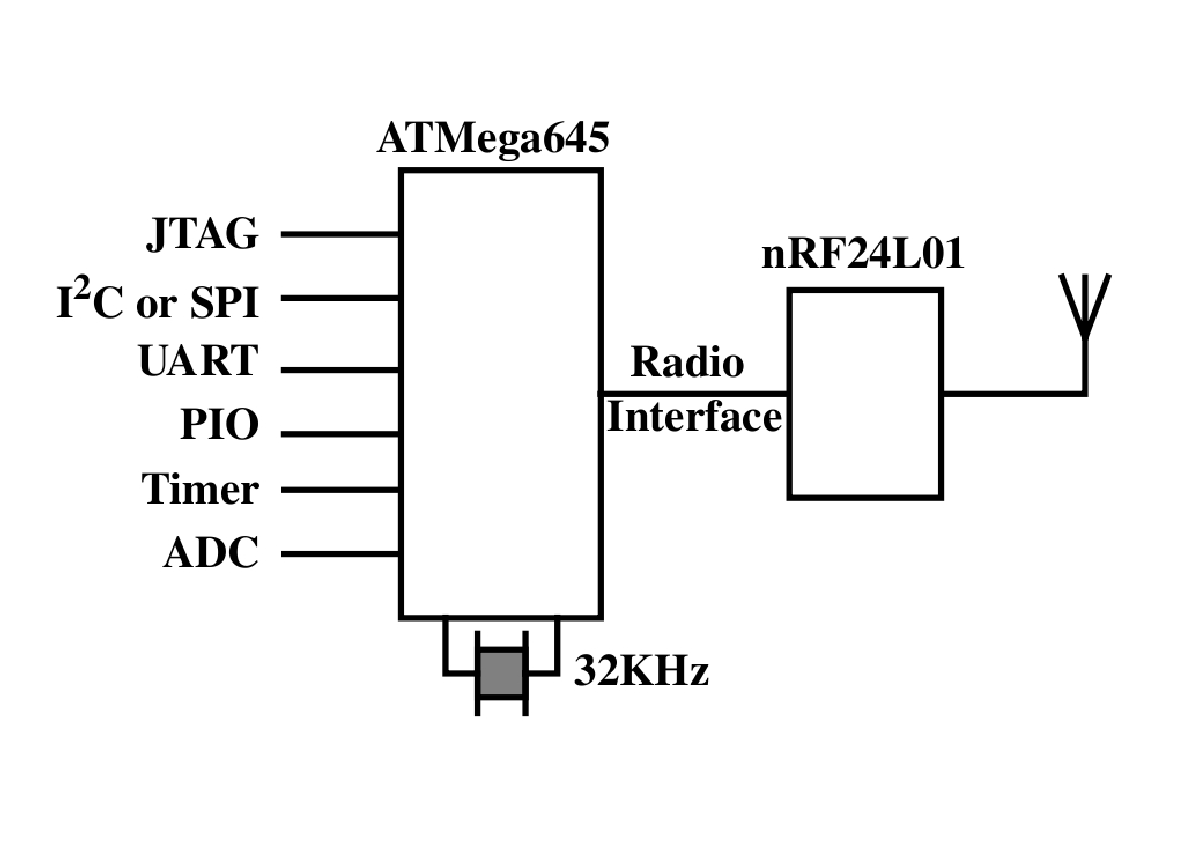
\includegraphics[width=0.5 \textwidth]{myrianodearch}
\caption{MyriaNode Architecure}
\label{myrianodearch}
\end{figure}
\subsection{Radio Interface}
SPI is used as interface between the processor and the radio, with the following interconnections:
\begin{figure}[!h]
 \centering
 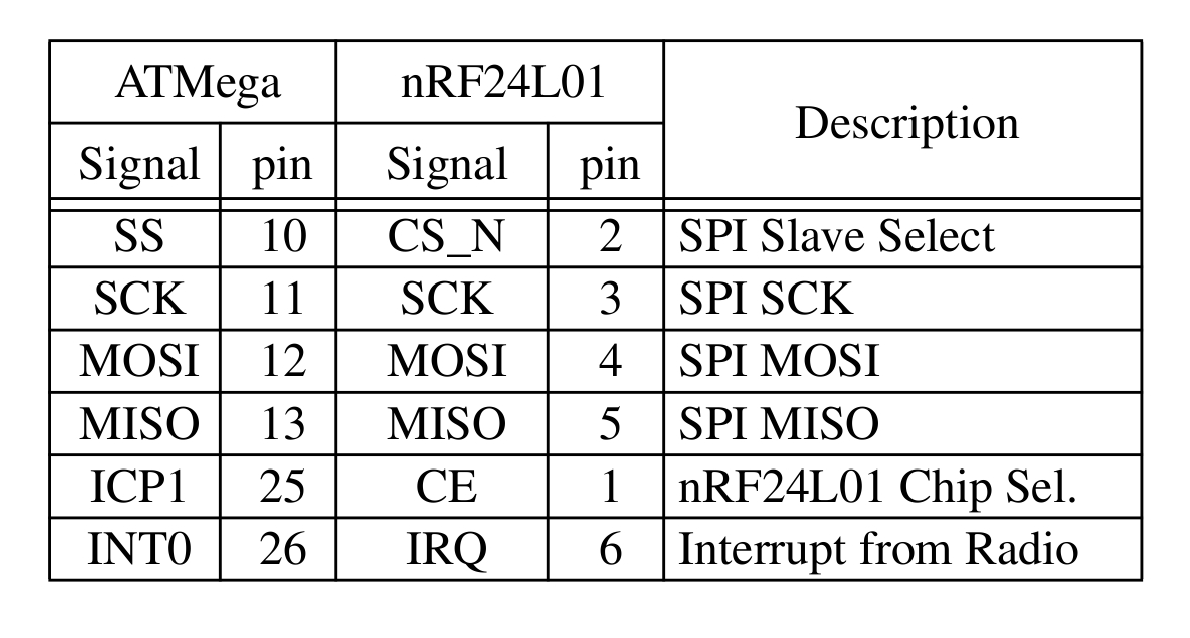
\includegraphics[width = 0.7 \textwidth] {table1}
 \caption{fad}
 \label{table1}
\end{figure}
\newline
\begin{figure}[!h]
 \centering
 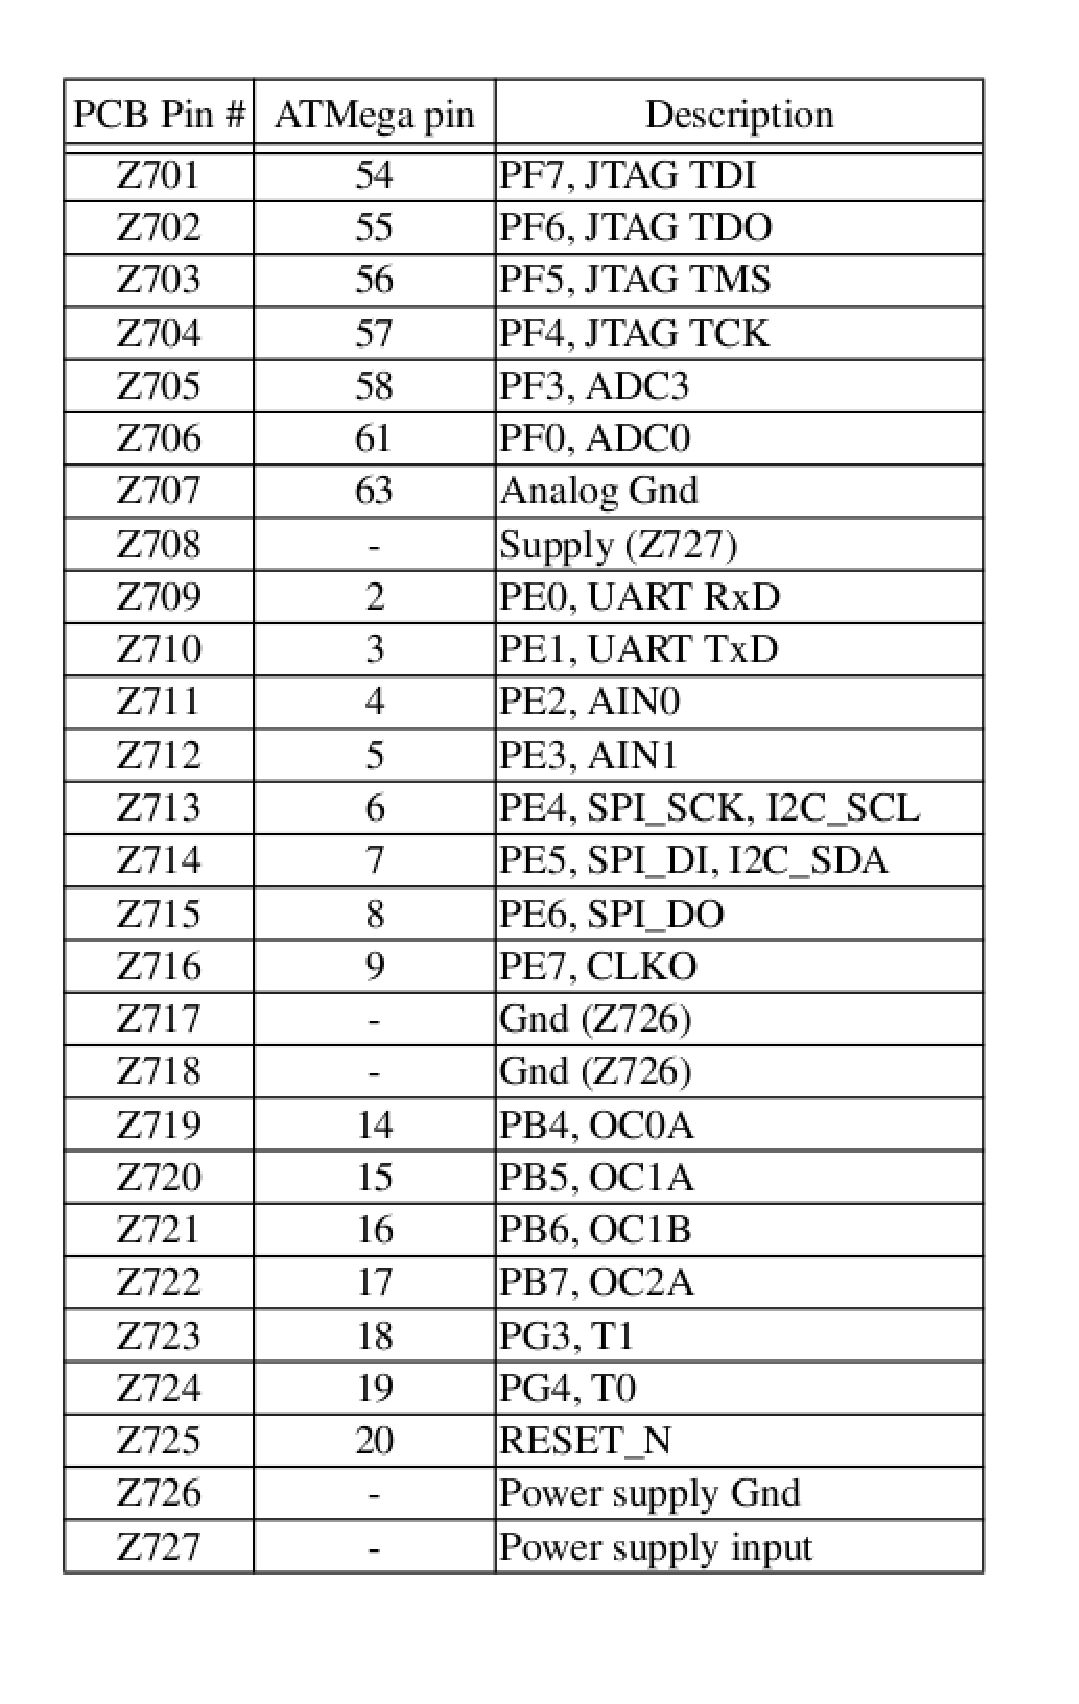
\includegraphics[width = 0.7 \textwidth] {table2}
 \caption{fdfa}
 \label{table2}
\end{figure}
\subsection{Mechanical and Mounting}
\begin{figure}[!h]
 \centering
 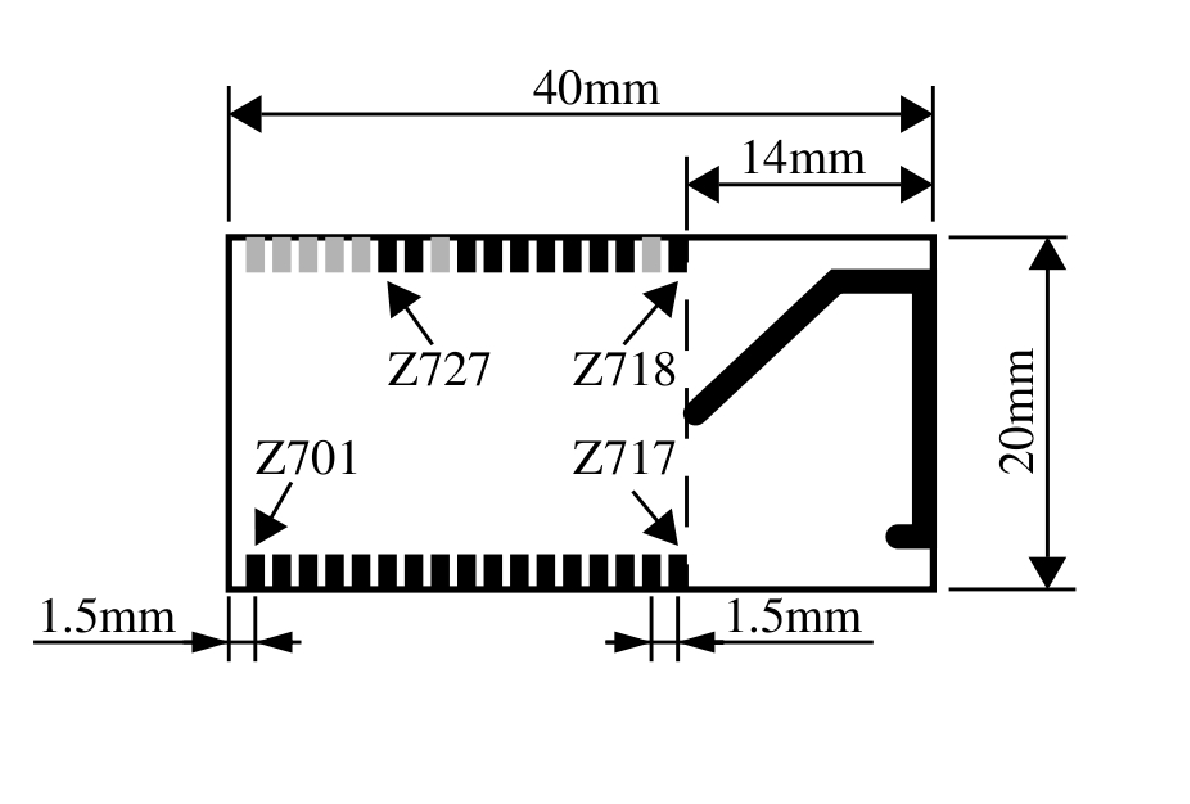
\includegraphics[width= 0.7 \textwidth]{myrianodephy}
 \caption{MyriaNode dimentions}
 \label{myrianodephy}
\end{figure}
Figure $\ref{myrianodephy}$ shows the top (component) view of the module. It can be mounted as a Surface Mount Device (SMD) directly onto a base PCB. The antenna area must be positioned in free air.
\subsection{Energy Supply}
Both the embedded processor and the radio are connected to the same supply rail. The supply voltage must therefore remain in a range that meet the supply voltage specifications of both devices, which is: 1.9V - 3.6V. \newline
Inorder to reduce conversion noise of the ADC to a minimum, the power decoupling circuit is implemented following the guidelines in the datasheet of the ATMega645. \newline
The energy consumption very much dependes on the network parameters and application software. Under average conditions of a network cycle time of 1s, and a frame size of 32 bytes, the node can last for at least 5 years on a Lithium Thionyl Chloride battery of 900mAh. \newline
The voltage level of a new Lithium Thionyl Chloride battery is 3.67V, while the absolute maximum operating voltage of the nRF24L01 is 3.60V. This requires a voltage reduction circuit. The most simple one is to connect the node via a diode to the battery, as is shown in the following figure:
\begin{figure}[!h]
 \centering
 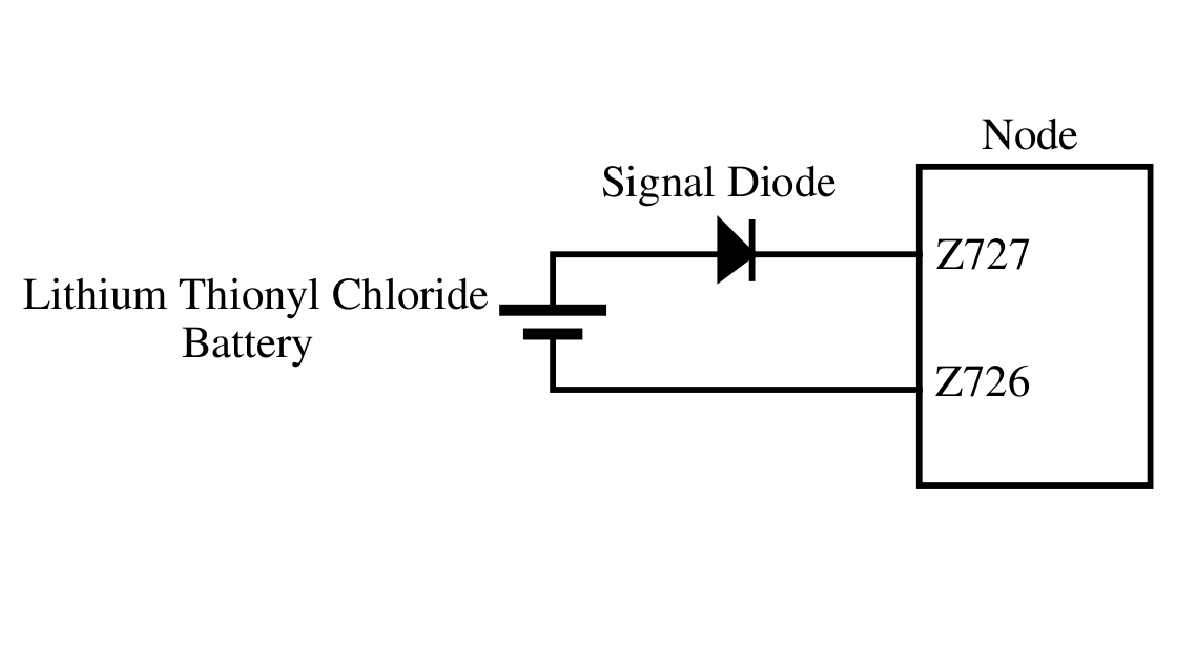
\includegraphics[width = 0.5 \textwidth]{battery}
 \caption{Battery structure of a MyriaNode}
 \label{battery}
\end{figure}
\subsection{Battery}
The ER14250STU from EMB is a good Lithium Thionyl Chloride battery. It has a form factor of 1/2 AA size, and has a capacity of 1000mAh.
\subsection{Programming}
The node can be programmed and debugged via the JTAG interface. Although there are many second source suppliers of JTAG development tools, it is advised to use the AVR JTAGICE mkII from Atmel, ordering code: ATJTAGICE2.
\subsection{Software}
The software is documented by the other working groups of MyriaNed.
\end{document}
